% Chapter 6 (English, standalone): solution methods and simulation results.
% Compile:  xelatex chapter6_en.tex   (twice, for references)
% Figures:  ./figures/  (made by oran_sim/scripts/plot_outputs.py)
% Lines marked TODO are to be updated when the full RL training grid has finished.
\documentclass[11pt,oneside]{report}
\usepackage[a4paper,margin=2.5cm]{geometry}
\usepackage{amsmath,amssymb}
\usepackage{graphicx}
\usepackage{booktabs}
\usepackage{float}
\usepackage{caption}
\usepackage{enumitem}
\usepackage[hidelinks]{hyperref}
\setlist{itemsep=2pt}
\setcounter{chapter}{5}

\newcommand{\cU}{\mathcal{U}}
\newcommand{\cB}{\mathcal{B}}
\newcommand{\cN}{\mathcal{N}}
\newcommand{\cM}{\mathcal{M}}

\begin{document}

\chapter{Solution Methods and Simulation Results}\label{ch:results}

This chapter solves the joint radio and computing resource allocation problem of an O-RAN network in two ways and compares the results.
The first is an optimisation-based method that finds the optimal solution together with a certified lower bound; it is the reference against which everything else is measured.
The second is a family of two-timescale deep reinforcement learning (RL) methods:
multi-agent RL with two TD3 agents (MARL),
a hybrid of one RL agent (TD3 or SAC) with convex optimisation,
and a single SAC agent.
Section~\ref{sec:setup} defines the network and the problem, Sections~\ref{sec:opt} and~\ref{sec:rl} describe the two solution families, and Sections~\ref{sec:res_opt}--\ref{sec:res_rl} present the results.

% =====================================================================================
\section{Network model and problem}\label{sec:setup}

\subsection{Network and traffic}
The network has $B=4$ radio units (RUs) on a regular grid in a $1000\times1000$\,m area, $|\cN^e|=4$ edge O-Cloud nodes and $|\cN^r|=2$ regional O-Cloud nodes.
Each RU has $M=25$ physical resource blocks (PRBs) sharing 25\,MHz and a maximum transmit power of 40\,dBm.
The channel gain of user $u$ on PRB $m$ of RU $b$ is $G_{b,u}h_{b,u,m}$, with log-distance path loss (exponent 3) and Rayleigh fading; the noise density is $-174$\,dBm/Hz and there is no inter-RU interference.
Users are dropped uniformly at random and split evenly over three slices (Table~\ref{tab:slices}).
The small timescale is one 1\,ms slot and the large timescale is $K=10$ slots.
Every result is averaged over five random drops (seeds) per user count $U\in\{5,10,15,20\}$.

\begin{table}[H]
	\centering
	\caption{Slice parameters.}\label{tab:slices}
	\begin{tabular}{lccccc}
		\toprule
		Slice & $D_s^{QoS}$ & packet size $q$ & arrival rate $\lambda$ & weight $\delta_s$ & speed \\
		\midrule
		eMBB  & 25\,ms   & 1500\,B & 100\,pkt/s & 0.5 & 1.5\,m/s \\
		URLLC & 5\,ms    & 200\,B  & 50\,pkt/s  & 0.9 & 1.5\,m/s \\
		mMTC  & 1000\,ms & 20\,B   & 1\,pkt/s   & 0.1 & static \\
		\bottomrule
	\end{tabular}
\end{table}

\paragraph{Computing and transport.}
The central unit (CU) and distributed unit (DU) of each RU are placed on O-Cloud nodes.
An edge node has one 3.4\,GHz core; a regional node has ten.
Processing $1$\,Mb/s needs $0.00175\times3.4$\,GHz at the CU and $0.04\times3.4$\,GHz at the DU, and one CPU cycle at the edge costs ten times as much as at a regional node.
Fronthaul (RU--DU) and midhaul (DU--CU) links carry $10\times$ and $1\times$ the user data rate over 100\,Gb/s and 10\,Gb/s fibre.

\paragraph{Three modelling choices.}
\begin{itemize}
	\item \textbf{Packet sizes are in bytes.} Reading them as kilobits overloads the transport links and makes every placement infeasible.
	\item \textbf{Each O-Cloud node is an $M/M/c$ queue} ($c$ = number of cores) with Erlang-C waiting time and per-packet service time $\tilde c^{\,l} q_u / f_{\text{core}}$. This makes the processing delay depend on where a function is placed. The fronthaul latency budget is 100\,$\mu$s.
	\item \textbf{Scheduling constraint:} if the CU and DU of an RU are on different nodes, CU$\to$DU propagation + CU processing + midhaul transmission must not exceed $\theta = 1$\,ms.
\end{itemize}

\subsection{Decision variables and delays}
The decisions are the user association $\alpha_{u}^{b}\in\{0,1\}$, the PRB assignment $\kappa_{u}^{b,m}\in\{0,1\}$, the PRB power $\omega_{u}^{b,m}\ge0$ and the placement $\psi_{b}^{l,n}\in\{0,1\}$ of function $l\in\{\mathrm{CU},\mathrm{DU}\}$ of RU $b$ on node $n$.
The rate of user $u$ is
\begin{equation}\label{eq:rate}
	R_u=\sum_{b}\alpha_u^b\sum_{m}\kappa_u^{b,m}\,B_p\log_2\!\Big(1+\frac{\omega_u^{b,m}G_{b,u}h_{b,u,m}}{N_0B_p}\Big),
\end{equation}
where $B_p$ is the PRB bandwidth.
The end-to-end delay of user $u$ served by RU $b$ is
\begin{equation}\label{eq:e2e}
	D_u^{e2e}=\underbrace{\frac{1}{R_u/q_u-\lambda_u}}_{\text{radio queue}}
	+\underbrace{D_b^{\text{proc}}}_{\text{node queues}}
	+\underbrace{D_b^{\text{tr}}}_{\text{fronthaul/midhaul}}
	+\underbrace{D_b^{\text{prop}}}_{\text{propagation}} .
\end{equation}
The cost $\bar\phi$ is the average CPU cost of the nodes hosting the functions.

\subsection{Optimisation problem}
Delay and cost are measured in very different units, so both terms are normalised:
\begin{equation}\label{eq:J}
	J=\sum_{s=1}^{3}\Big(\delta_s\,\frac{1}{|\cU_s|}\sum_{u\in\cU_s}\frac{D_u^{e2e}}{D_s^{QoS}}+(1-\delta_s)\frac{\bar\phi}{\phi_{\max}}\Big),\qquad \phi_{\max}=2\max_n\phi_n .
\end{equation}
$J$ has no unit. A delay term of 1 means the user is exactly at its slice's QoS budget.
Equivalently, $J=\sum_u w_uD_u^{e2e}+K\bar\phi$ with $w_u=\delta_s/(|\cU_s|D_s^{QoS})$.
The problem is
\begin{equation}\label{eq:problem}
	\min_{\alpha,\kappa,\omega,\psi}\ J
	\quad\text{s.t.}\quad
	\begin{cases}
		\sum_b\alpha_u^b=1, \quad \kappa_u^{b,m}\le\alpha_u^b, \quad \sum_u\kappa_u^{b,m}\le1 & \text{(association, PRBs)}\\
		\sum_{u,m}\kappa_u^{b,m}\omega_u^{b,m}\le P_b^{\max} & \text{(power)}\\
		\sum_n\psi_b^{l,n}=1,\quad \text{CPU and link capacities} & \text{(placement)}\\
		\text{all queues stable},\ D_u^{e2e}\le D_s^{QoS} & \text{(QoS)}\\
		\text{fronthaul budget},\ \text{scheduling constraint } \theta & \text{(timing)}
	\end{cases}
\end{equation}
This is a mixed-integer nonlinear program (MINLP).

% =====================================================================================
\section{Optimisation-based solution}\label{sec:opt}

\paragraph{Exact decomposition.}
With no interference, a user's rate depends only on the PRBs and power of its own RU.
For a fixed association $\alpha$ the objective therefore splits exactly into
\begin{equation}\label{eq:decomp}
	J=\sum_{b\in\cB}V_b\big(\kappa_b,\omega_b;\alpha,\sigma_b\big)+I(\psi;\alpha),
\end{equation}
where:
\begin{itemize}
	\item $V_b$ holds the rate-dependent terms of RU $b$: the radio queue and the fronthaul/midhaul transmission delay.
	\item $V_b$ depends on the placement only through $\sigma_b=\mathbb{1}[\text{CU and DU of } b \text{ on different nodes}]$.
	\item $I$ holds the rate-independent terms: propagation, node queues and cost.
\end{itemize}
For each association it is enough to solve two radio problems per RU, for $\sigma_b=0$ and $\sigma_b=1$, and then optimise the placement over the stored values.
The solver has four layers.

\paragraph{1. Power allocation (convex, globally optimal).}
For a fixed PRB assignment, each $R_u$ is concave in the powers and $1/(R_u/q_u-\lambda_u)$ is convex and decreasing in $R_u$, so $V_b$ is convex in $\omega$.
Each iteration does three things:
\begin{enumerate}
	\item Linearise $V_b$ in the rates, with weights $\kappa_u=-\partial V_b/\partial R_u>0$.
	\item Solve the resulting weighted sum-rate problem exactly by water-filling:
	\begin{equation}\label{eq:wf}
		p_m=\Big[\frac{\kappa_{o(m)}B_p}{\mu\ln2}-\frac{1}{a_m}\Big]^+,\qquad \sum_mp_m=P_b^{\max},
	\end{equation}
	where $o(m)$ is the owner of PRB $m$, $a_m$ its gain-to-noise ratio, and $\mu$ the power price, found in closed form over the sorted PRBs.
	\item Take an exact line search towards that point.
\end{enumerate}
A fixed point of this procedure satisfies the KKT conditions, so it is the global optimum. In tests it was never worse than the generic conic solver Clarabel (via CVXPY).

\paragraph{2. PRB assignment (combinatorial).}
Small RUs are enumerated exhaustively. Otherwise the solver:
\begin{enumerate}
	\item builds a greedy assignment from marginal gains;
	\item improves it by single-PRB moves;
	\item refines it with \emph{exact moves}: the 12 best candidate moves (one PRB moved, or two PRBs swapped between users) are re-evaluated with optimal power, and the best real improvement is kept until none improves.
\end{enumerate}
Every associated user keeps at least one PRB; otherwise its radio queue would be unstable.

\paragraph{3. CU/DU placement (exhaustive).}
Given $\alpha$ and the stored $V_b(\sigma_b)$, a placement is evaluated by arithmetic alone.
All $N^{2B}=6^8=1\,679\,616$ placements are enumerated in vectorised form in a few seconds, with every CPU, link, queue-stability and timing constraint checked.
The placement is therefore exactly optimal for each association.

\paragraph{4. User association (multi-start local search).}
There are $B^U$ associations ($4^{20}\approx10^{12}$ at $U=20$).
The search runs from 8 starts: the best-channel association, plus random mixes of each user's two or three best RUs.
Each move transfers one user to another of its three best RUs and is accepted if $J$ (with re-optimised placement) decreases.
The best result is refined and its placement re-optimised exhaustively.

\paragraph{Certified lower bound.}
Relaxing PRBs and association to fractions and using the perspective rate $x\,B_p\log_2(1+a\,s/x)$ gives a convex problem.
Its Lagrangian dual has a closed form per (RU, PRB, user). By weak duality, any multipliers give a valid lower bound; the multipliers are maximised with L-BFGS on a smoothed dual that is itself a valid bound. Two gaps are reported:
\begin{itemize}
	\item \textbf{conditional gap:} over all PRB, power and placement choices, for the association found;
	\item \textbf{global gap:} with the association relaxed as well. This bound loosens as $U$ grows, so it is a conservative upper limit on the true gap.
\end{itemize}

\paragraph{Validation.}
On 12 small instances ($B=N=2$, $U=M=3$) where every variable can be enumerated, the scalable solver found the exact global optimum in \textbf{12 of 12} cases.
In unit tests, the decomposition~\eqref{eq:decomp} matches a direct evaluation of all KPIs.

% =====================================================================================
\section{Two-timescale reinforcement learning}\label{sec:rl}
The problem is cast as a two-timescale Markov decision process. Every slot, the small timescale decides PRBs and power $(\kappa,\omega)$; every $K=10$ slots, the large timescale decides association and placement $(\alpha,\psi)$.
An episode is 10 large steps (100 slots).
Each training episode draws a new user drop on the fixed network.
The trained policy, without exploration noise, is evaluated on the same instance for which the optimum was computed, so the two can be compared directly.

\paragraph{State.}
The large-timescale state is
\begin{equation}\label{eq:sL}
	s^L_t=\Big[\tfrac{1}{40}\big(10\log_{10}G_{b,u}+120\big),\ \mathbf e^{\text{slice}}_u,\ \mathbf e^{\alpha}_u,\ \mathbf e^{\mathrm{CU}}_b,\ \mathbf e^{\mathrm{DU}}_b,\ \rho_n,\ \phi_n/\phi_{\max}\Big],
\end{equation}
It contains:
\begin{itemize}
	\item the normalised large-scale gains of all (RU, user) pairs;
	\item one-hot vectors for each user's slice and current RU;
	\item one-hot vectors for the current CU and DU node of each RU;
	\item the CPU utilisation $\rho_n$ and cost of every node.
\end{itemize}
The small-timescale state adds the fading of each user on every PRB of its serving RU: $s^S_t=[s^L_t,\ 10\log_{10}h_{b(u),u,m}/10]$.
For $U=10$, $\dim s^L=170$ and $\dim s^S=420$; for $U=20$ they are 280 and 780.

\paragraph{Action and decoding.}
Actions are continuous in $[-1,1]$. They are decoded so that association, PRB exclusivity, power and placement constraints always hold.
\begin{itemize}
	\item \textbf{Large action} $a^L\in[-1,1]^{UB+2BN}$ (88 at $U=10$): one score per (user, RU) pair and one per (RU, node) pair for each of CU and DU. The decision is the arg-max of score plus a \emph{residual prior}:
	\begin{equation}\label{eq:decL}
		b(u)=\arg\max_b\big(a^L_{u,b}+\beta\,\mathbf{1}[b=b^{\text{st}}(u)]\big),\qquad
		n^l(b)=\arg\max_n\big(a^L_{l,b,n}+\beta\,\mathbf{1}[n=n^{l,\text{st}}(b)]\big).
	\end{equation}
	Here $(b^{\text{st}},n^{\text{st}})$ is the best static decision: best-channel association with the best static placement scenario.
	A zero action therefore reproduces the static baseline, and the agent only has to learn deviations that pay off.
	\item \textbf{Small action} $a^S=[z,y]\in[-1,1]^{2U}$: within each RU:
	\begin{itemize}
		\item PRB shares are $\pi_u=\mathrm{softmax}(\tau z)_u$ and power shares are $\varpi_u=\mathrm{softmax}(\tau y)_u$;
		\item PRB counts come from the largest-remainder method, with at least one PRB per user;
		\item PRBs are dealt to users in order of channel quality;
		\item each user's power is split evenly over its PRBs, and the RU always uses its full power $P_b^{\max}$.
	\end{itemize}
\end{itemize}

\paragraph{Reward.}
All agents share the reward
\begin{equation}\label{eq:reward}
	r_t=-\min\Big\{\frac{J_t+\varrho\,N^{\text{viol}}_t\,J_{\text{ref}}}{J_{\text{ref}}},\ r_{\max}\Big\}-c_a\,\overline{a_t^{2}},
\end{equation}
where:
\begin{itemize}
	\item $J_t$ is the objective~\eqref{eq:J};
	\item $N^{\text{viol}}_t$ is the number of violated constraints (capacity, queue stability, QoS, fronthaul budget, scheduling);
	\item $J_{\text{ref}}$ is the objective of the best static scenario for the current drop;
	\item $\varrho=1$ and $r_{\max}=10$;
	\item $\overline{a_t^2}$ is the mean squared action that was applied.
\end{itemize}
With this scaling the static baseline earns about $-1$ and the optimum $-J^*/J_{\text{ref}}>-1$.
The large agent's reward is the mean over its $K$ slots (a semi-MDP transition).
Episodes end only by time limit, so transitions are stored as non-terminal.

\paragraph{Methods compared.}
\begin{itemize}
	\item \textbf{MARL (2$\times$TD3):} one TD3 agent per timescale. The small agent's critic also sees the current large action (centralised training, decentralised execution).
	\item \textbf{Hybrid (TD3 or SAC + convex):} the RL agent decides only association and placement. Every slot, PRBs come from local search and power from~\eqref{eq:wf} (40 iterations).
	\item \textbf{Single SAC:} one agent outputs $[a^L,a^S]$ every slot; $a^L$ is applied at the start of each $K$-slot period.
\end{itemize}

\begin{table}[H]
	\centering
	\caption{RL hyper-parameters.}\label{tab:rl}
	\begin{tabular}{p{8.5cm}p{5.5cm}}
		\toprule
		Parameter & Value \\
		\midrule
		Actor / critic hidden layers (small agent) & (1024, 512) / (512, 256) \\
		Actor / critic learning rate & $10^{-4}$ / $10^{-3}$ \\
		Discount $\gamma$, soft update $\tau_{\text{soft}}$ & 0.99, 0.005 \\
		Replay buffer; batch (small / large agent) & 50\,000; 128 / 64 \\
		Random warm-up transitions (small / large) & 500 / 50 \\
		TD3 exploration / target noise, clip, policy delay & 0.1 / 0.2, 0.5, 2 \\
		SAC initial temperature (auto-tuned) & 0.2 \\
		Residual prior $\beta$; share factor $\tau$; action penalty $c_a$ & 1; 1; 0.1 \quad (TODO: confirm) \\
		Large agent: layers, gradient steps per transition & (1024, 512), 10 \quad (TODO: confirm) \\
		Episodes $\times$ slots & 1000 $\times$ 100 \\
		\bottomrule
	\end{tabular}
\end{table}

% =====================================================================================
\section{Results: optimum versus static baselines}\label{sec:res_opt}
Table~\ref{tab:p5} and Fig.~\ref{fig:p5} compare the optimum with the following baselines:
\begin{itemize}
	\item three static placements: all functions at the edge; CU regional and DU at the edge; all regional;
	\item the best of these three for each drop (best static);
	\item placement search: the placement optimised with the best-channel association kept fixed.
\end{itemize}

\begin{table}[H]
	\centering
	\caption{Normalised objective $J$ (mean of five drops). Gain = improvement over best static.}\label{tab:p5}
	\resizebox{\textwidth}{!}{%
	\begin{tabular}{ccccccccc}
		\toprule
		$U$ & all edge & CU reg./DU edge & best static & placement search & \textbf{optimum} & gain & cond.\ gap & global gap \\
		\midrule
		5  & 0.1806 & 0.1186 & 0.0561 & 0.0355 & \textbf{0.0310} & 33.2\% & 0.001\% & 4.5\% \\
		10 & 0.3416 & 0.2032 & 0.0432 & 0.0413 & \textbf{0.0344} & 19.5\% & 0.35\%  & 7.1\% \\
		15 & 0.4305 & 0.2502 & 0.0487 & 0.0479 & \textbf{0.0384} & 20.8\% & 1.51\%  & 10.0\% \\
		20 & 0.5923 & 0.3350 & 0.0525 & 0.0520 & \textbf{0.0426} & 18.5\% & 0.26\%  & 11.3\% \\
		\bottomrule
	\end{tabular}}
\end{table}

\begin{figure}[H]
	\centering
	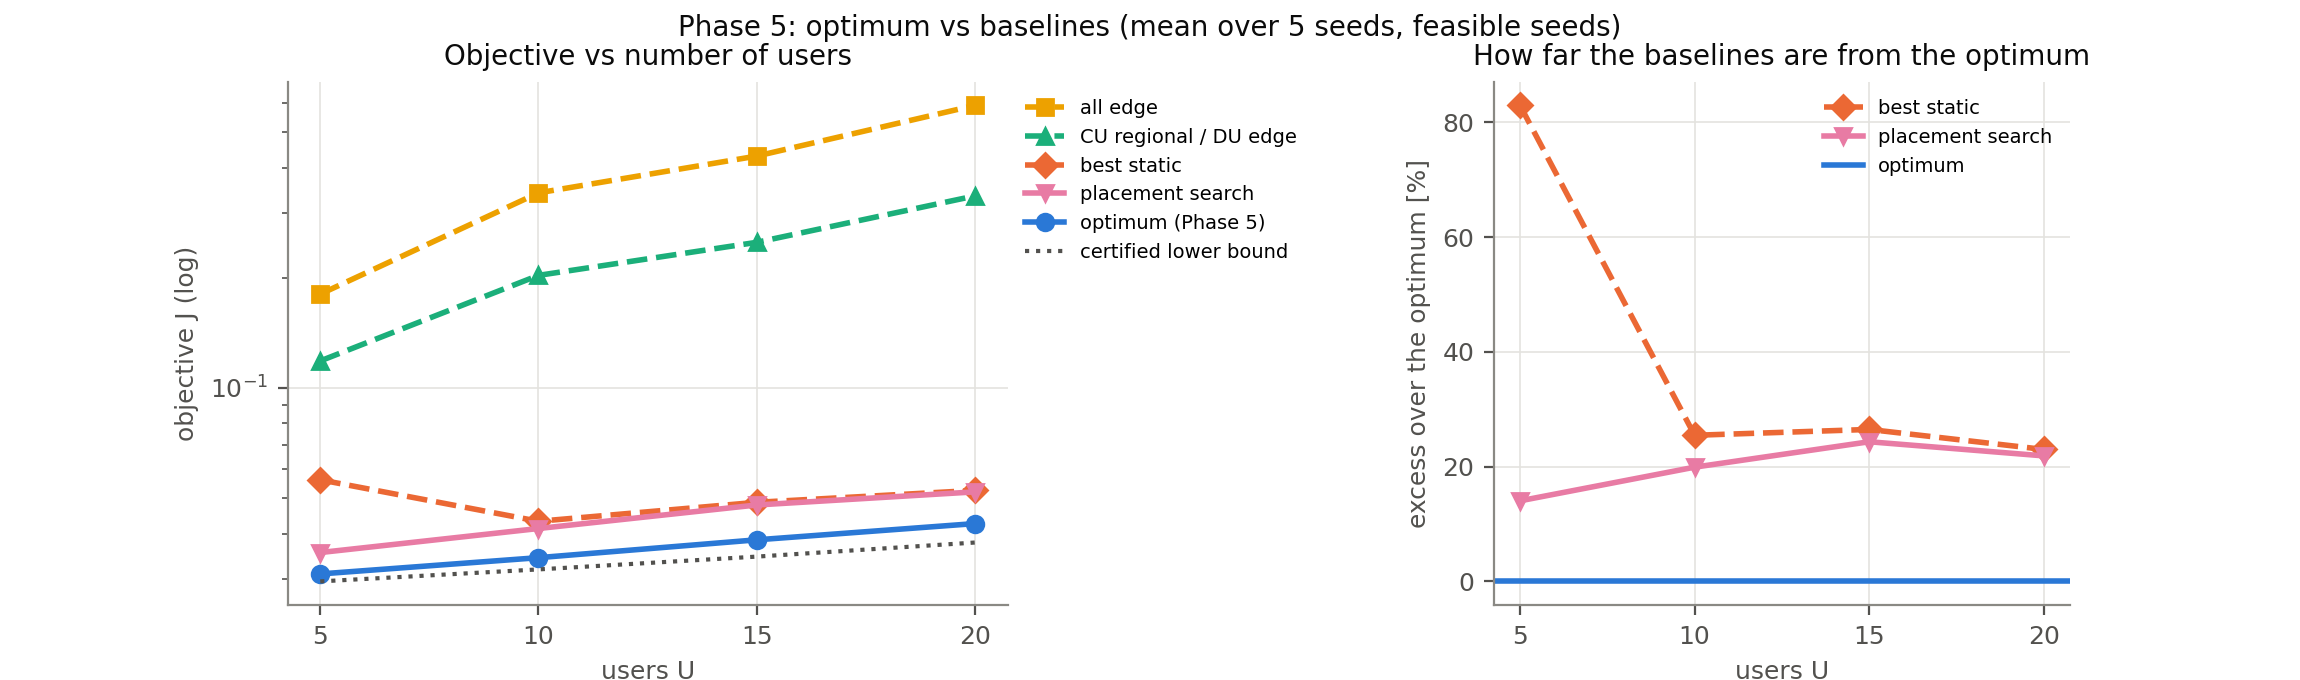
\includegraphics[width=\textwidth]{figures/phase5_optimum_vs_baselines.png}
	\caption{Left: objective of the optimum, the baselines and the certified lower bound versus the number of users. Right: excess of the baselines over the optimum.}\label{fig:p5}
\end{figure}

\begin{itemize}
	\item \textbf{The optimum beats the best static scenario in every drop}, by 18.5--33.2\% on average. The $U=5$ figure is inflated by one drop where the all-regional scenario breaks a capacity constraint, leaving a much weaker static fallback; without that drop the gain is about 12\%.
	\item \textbf{Optimising placement alone recovers little of this gain} (14--24\% above the optimum). Association, PRBs, power and placement must be optimised together.
	\item \textbf{Edge-only scenarios are 4--14 times worse.} A single edge core builds long processing queues, and an edge CPU cycle costs ten times more.
	\item \textbf{The conditional gap is below 0.4\%} (1.5\% at $U=15$): for the association found, PRBs, power and placement are essentially optimal. The global gap (4.5--11.3\%) grows because the relaxed-association bound loosens, so it overstates the true gap.
	\item \textbf{Solve time grows fast}: about 6\,min at $U=5$, 47\,min at $U=10$, several hours at $U\ge15$. This is far too slow for slot-by-slot decisions, which is the reason for learning a policy.
\end{itemize}

% =====================================================================================
\section{Results: system entities at the optimum}\label{sec:res_ent}
This section examines the instance $U=20$ (drop 0) in detail.

\paragraph{User association and placement.}
Fig.~\ref{fig:assoc} shows that the optimum does not simply attach users to their strongest RU: 6 of the 20 users, two from each slice, are attached elsewhere.
The heavy eMBB and URLLC users are balanced over the RUs (2--5 per RU), while six light mMTC users are gathered on RU4.
Here the CU and DU of every RU share one regional node: ten cores keep the processing queue short and cheap, and splitting CU and DU would add midhaul delay.
Across all drops, CU/DU splitting is never chosen for $U\le10$ and is chosen for 25--50\% of RUs at $U\ge15$.
The share of functions at the edge falls from 65\% ($U=5$) to 35\% ($U=20$) as the load grows.

\begin{figure}[H]
	\centering
	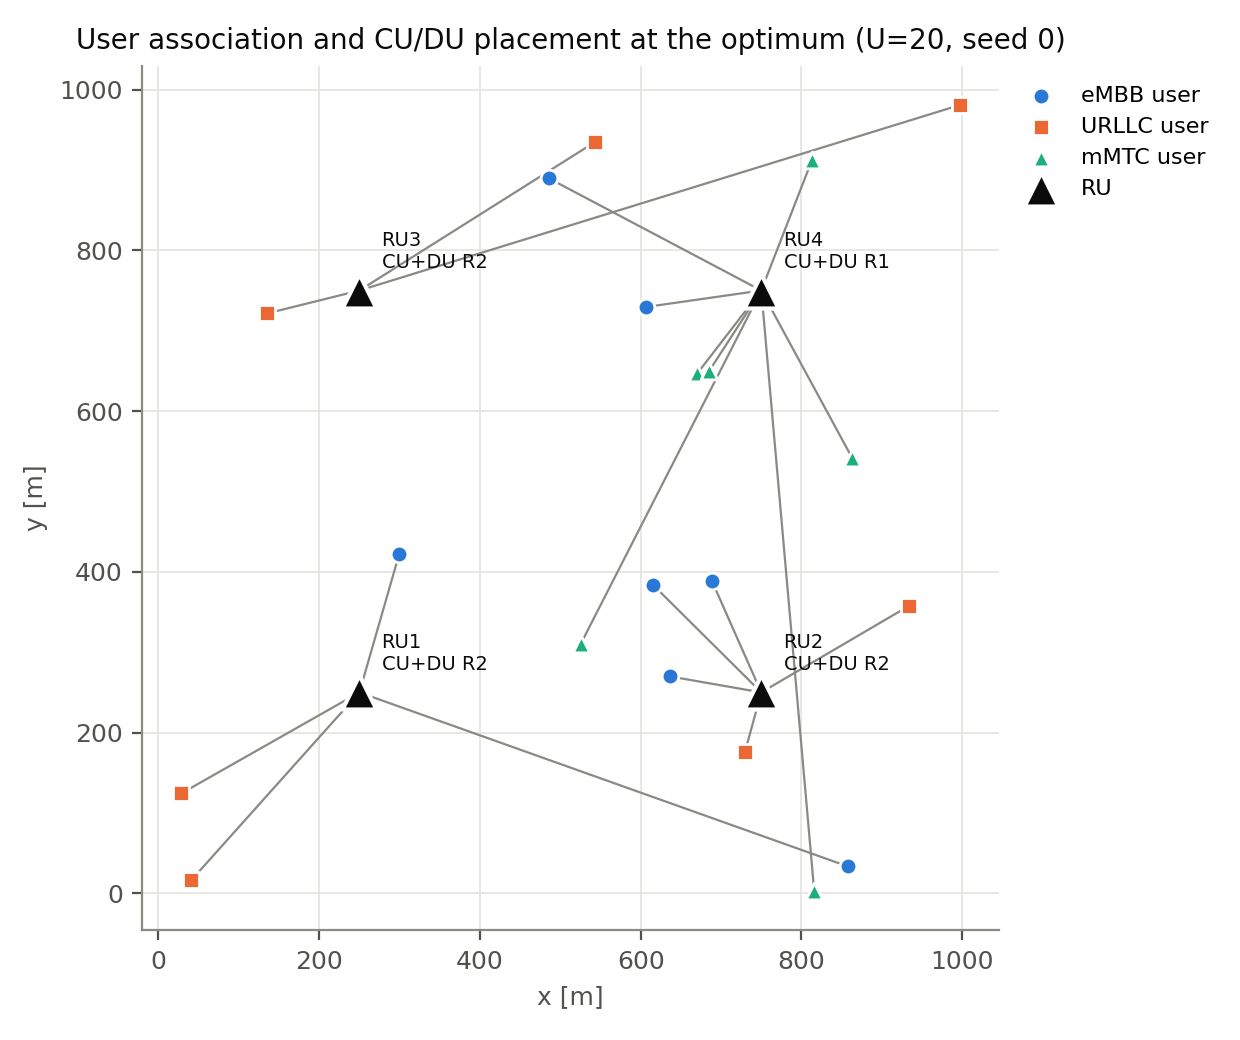
\includegraphics[width=0.78\textwidth]{figures/system_association.png}
	\caption{User association and CU/DU placement at the optimum ($U=20$).}\label{fig:assoc}
\end{figure}

\paragraph{Power and PRBs.}
Fig.~\ref{fig:power} shows the following:
\begin{itemize}
	\item eMBB and URLLC users receive 5--10 PRBs and 1--6\,W each;
	\item each mMTC user gets a single PRB at about 0.03\,W, enough to keep its queue stable;
	\item within each RU, power follows the water-filling rule~\eqref{eq:wf}: weaker PRBs receive less power or go to light users.
\end{itemize}

\begin{figure}[H]
	\centering
	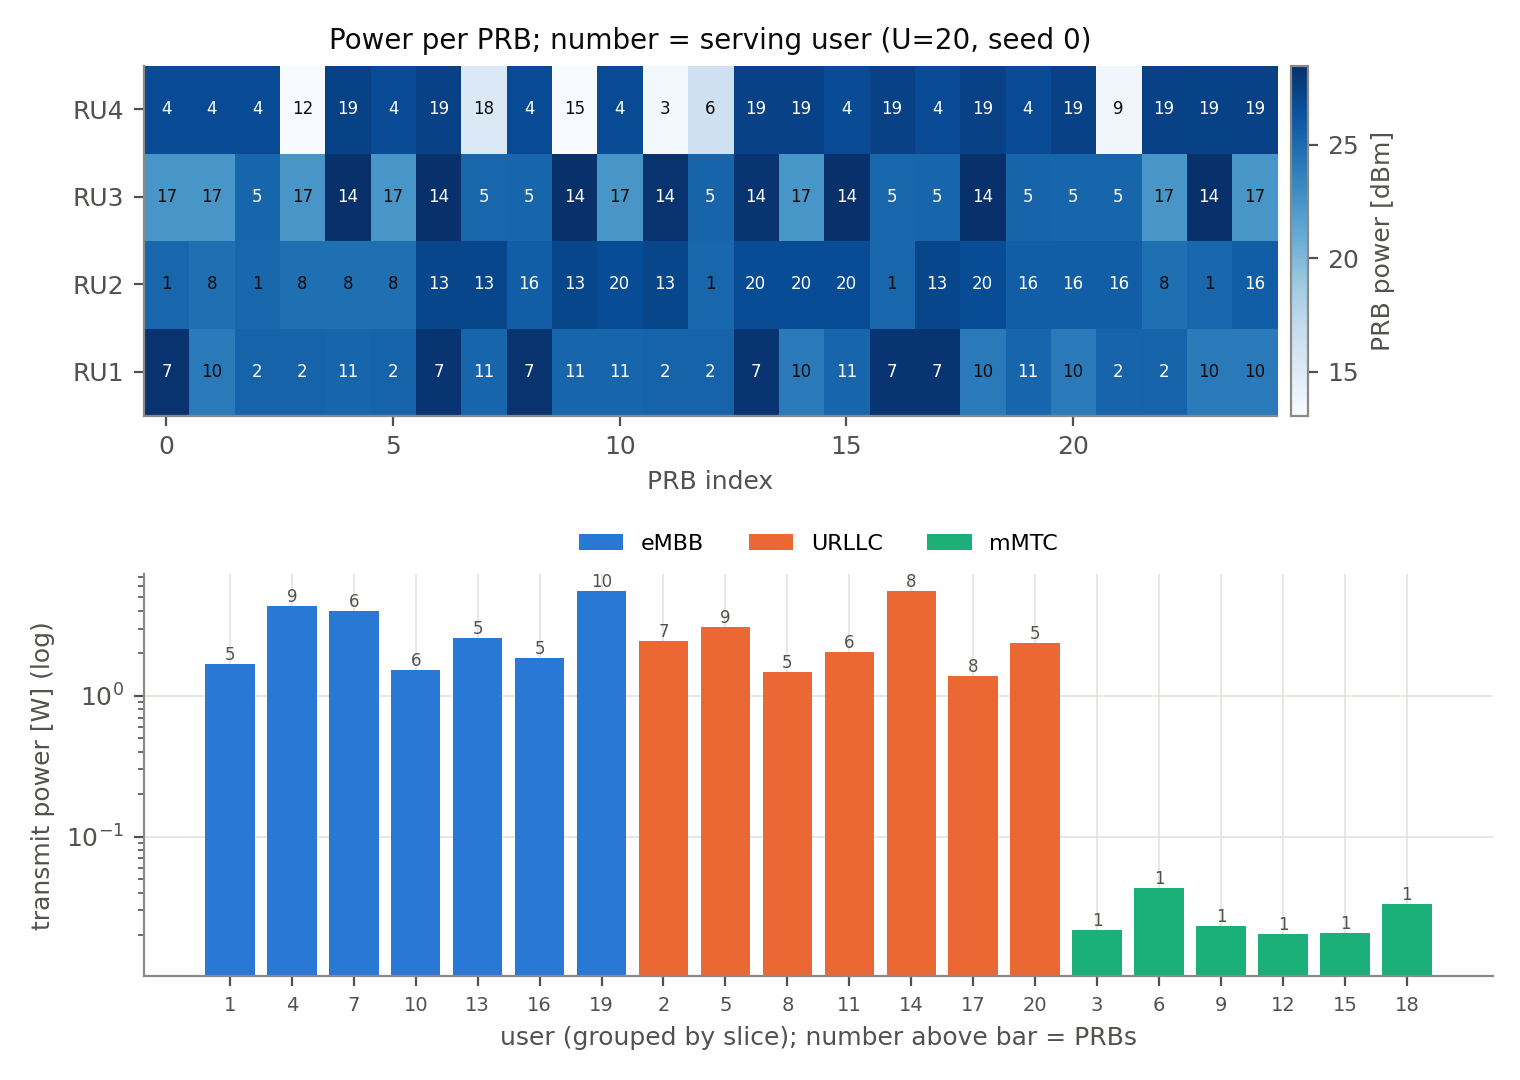
\includegraphics[width=0.9\textwidth]{figures/system_power.png}
	\caption{Top: power on each PRB (number = serving user). Bottom: total power and PRB count per user, grouped by slice.}\label{fig:power}
\end{figure}

\paragraph{Delay.}
Fig.~\ref{fig:delay} splits each user's end-to-end delay into its components:
\begin{itemize}
	\item \textbf{eMBB:} processing dominates (about 70\%), because 1500-byte packets need many CPU cycles.
	\item \textbf{URLLC:} processing is also the largest part (about 55\%), followed by the radio queue and propagation.
	\item \textbf{mMTC:} propagation dominates.
	\item \textbf{QoS:} every user is far below its budget: at most 0.87\,ms against 25\,ms for eMBB, and about 0.13\,ms against 5\,ms for URLLC.
\end{itemize}

\begin{figure}[H]
	\centering
	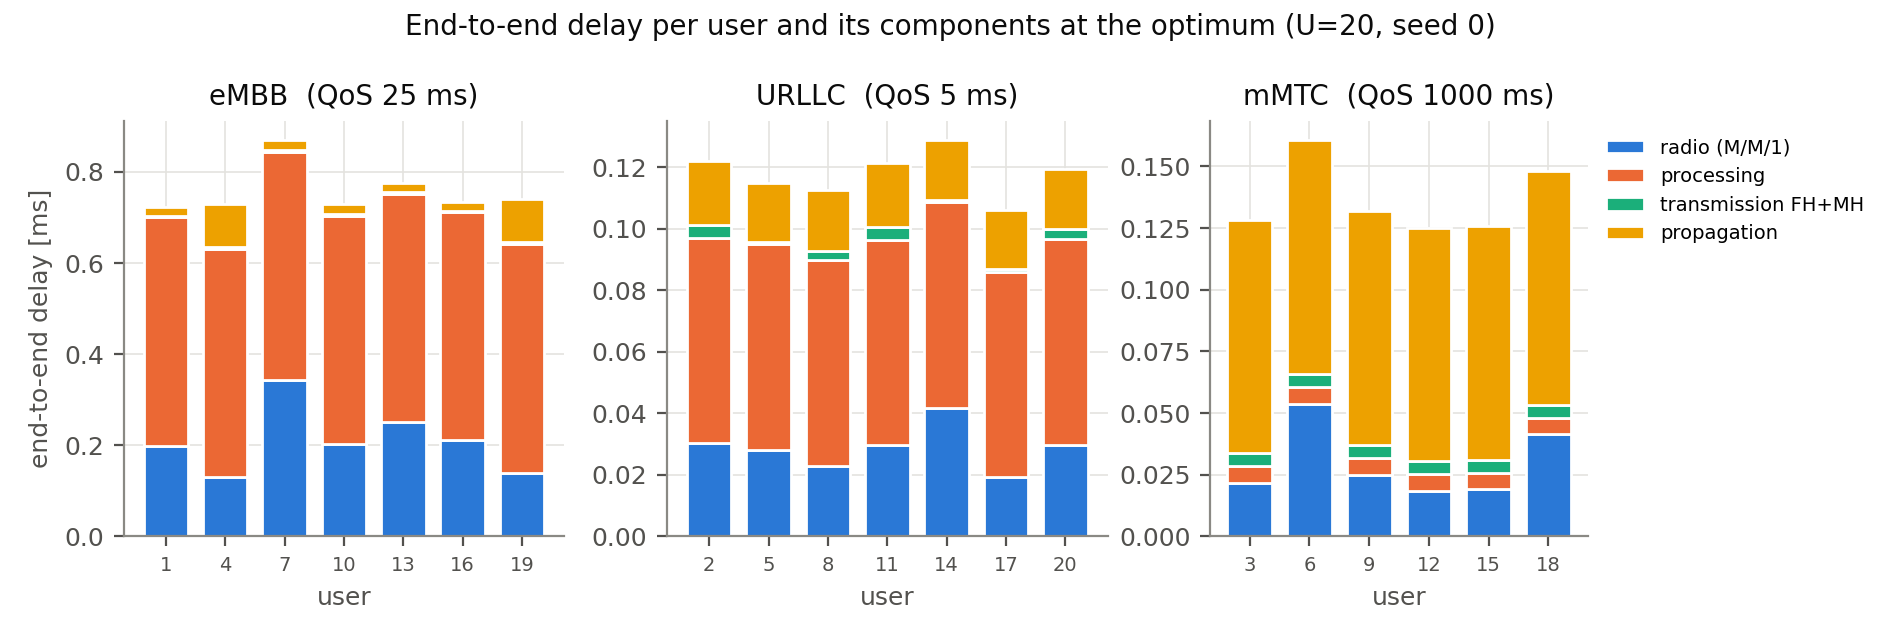
\includegraphics[width=\textwidth]{figures/system_delay.png}
	\caption{End-to-end delay per user and its components at the optimum.}\label{fig:delay}
\end{figure}

\paragraph{Processing power.}
Fig.~\ref{fig:proc} shows that the optimum splits the load over both regional nodes, cutting the peak CPU utilisation from 3.7\% to 2.7\% and shortening the processing queue.
The low utilisation shows that regional capacity is not the bottleneck; the per-packet service time and the cost of edge nodes are.

\begin{figure}[H]
	\centering
	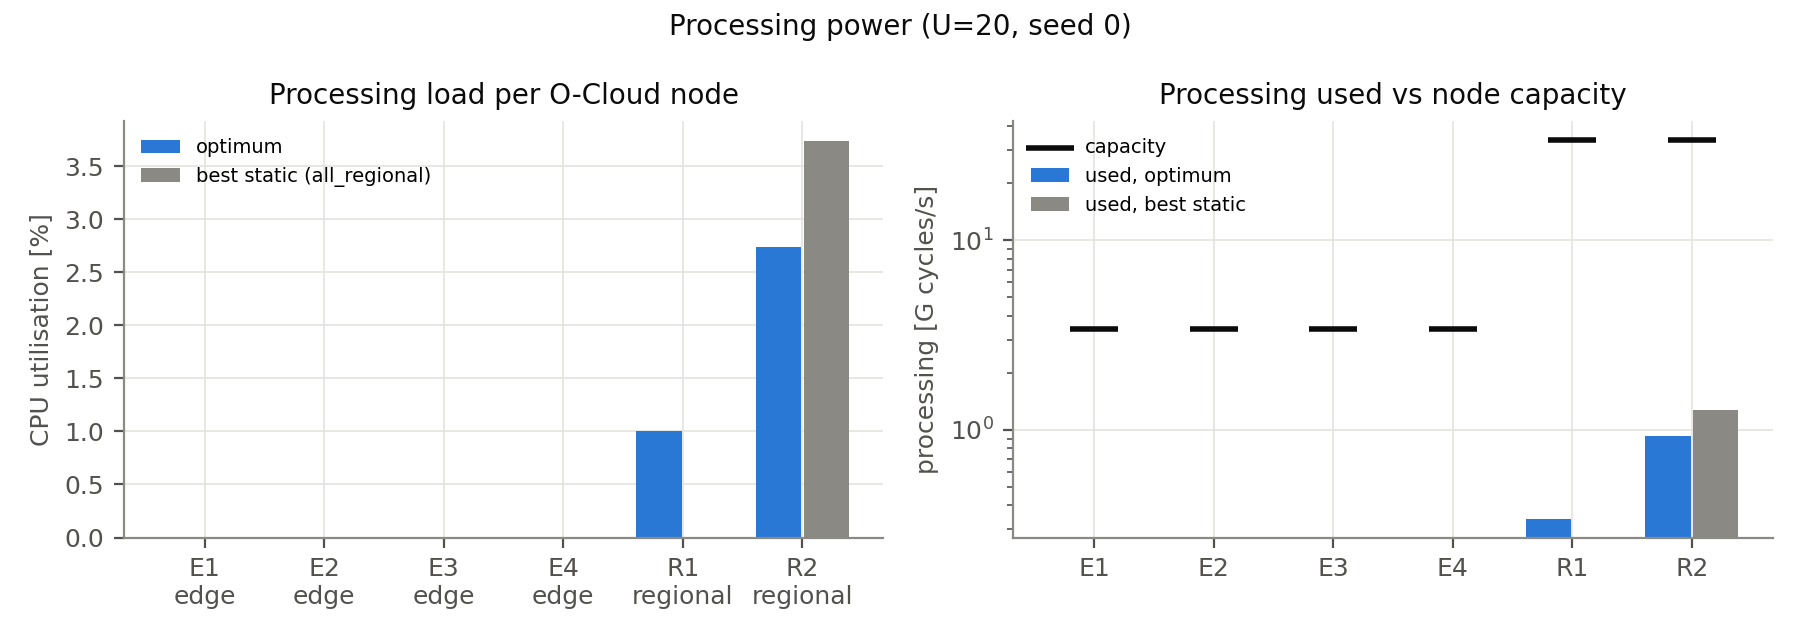
\includegraphics[width=\textwidth]{figures/system_processing.png}
	\caption{CPU utilisation and processing used per O-Cloud node, against capacity.}\label{fig:proc}
\end{figure}

\paragraph{How each slice reacts.}
Fig.~\ref{fig:slices} shows how each slice responds as the load grows:
\begin{itemize}
	\item \textbf{eMBB and URLLC:} delay rises with load under both the optimum and the best static scenario, but the optimum keeps URLLC delay 28--41\% lower.
	\item \textbf{mMTC:} for $U\ge10$ its delay is slightly higher at the optimum (0.09 against 0.065\,ms at $U=20$). This follows directly from its low weight ($\delta=0.1$): the optimiser shifts resources to the delay-sensitive slices.
	\item \textbf{Rates:} every slice receives several times its offered load, so all radio queues are stable and QoS is met for 100\% of users.
\end{itemize}

\begin{figure}[H]
	\centering
	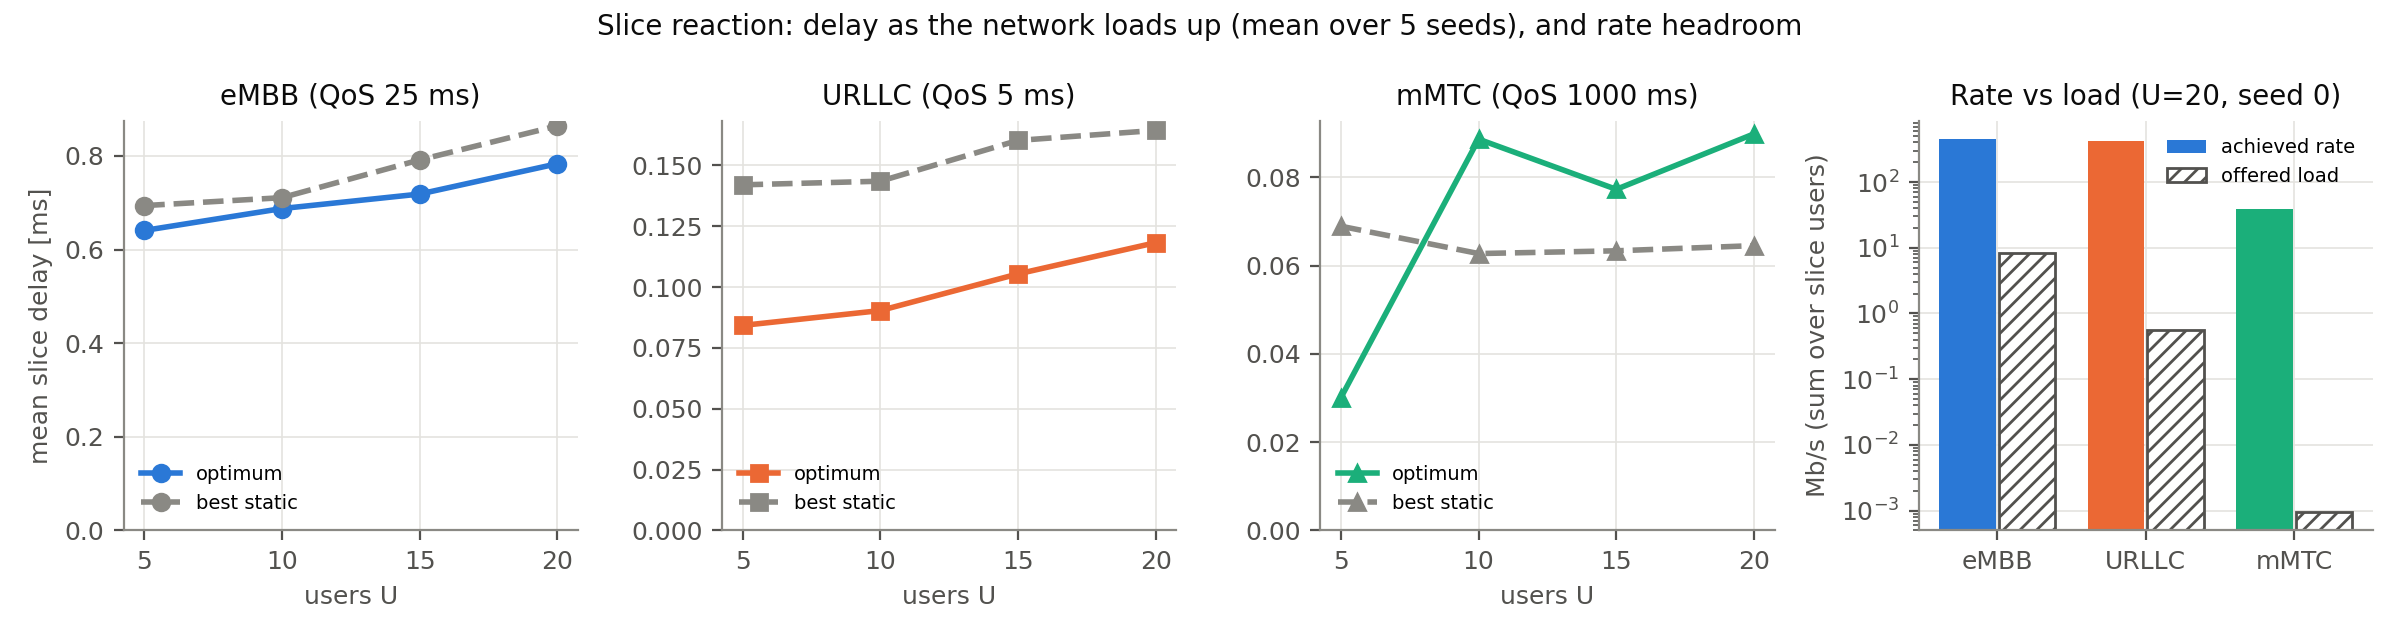
\includegraphics[width=\textwidth]{figures/system_slices.png}
	\caption{Mean slice delay versus number of users (optimum vs.\ best static), and achieved rate versus offered load.}\label{fig:slices}
\end{figure}

% =====================================================================================
\section{Results: reinforcement learning}\label{sec:res_rl}
% TODO: replace with the full grid (4 methods x U in {5,10,15,20} x 3 seeds x 1000 episodes).
These results are \textbf{preliminary}: a pilot run at $U=5$ with 150 episodes, on the instance for which the optimum is known.
The metric is the gap of the trained policy, without exploration, to the optimum.

\begin{table}[H]
	\centering
	\caption{Best trained policy versus the optimum (pilot, $U=5$, 150 episodes).}\label{tab:rl_pilot}
	\begin{tabular}{lccc}
		\toprule
		Method & without prior & with residual prior & $J$ (with prior) \\
		\midrule
		TD3 + convex          & +12.4\% & \textbf{+2.2\%} & 0.0308 \\
		SAC + convex          & +26.2\% & +5.9\%  & 0.0319 \\
		MARL (2$\times$TD3)   & +54.2\% & +7.2\%  & 0.0323 \\
		single SAC            & +150\%  & +12.0\% & 0.0337 \\
		\midrule
		best static           & \multicolumn{2}{c}{+13.2\%} & 0.0341 \\
		optimum               & \multicolumn{2}{c}{0}       & 0.0301 \\
		\bottomrule
	\end{tabular}
\end{table}

\begin{figure}[H]
	\centering
	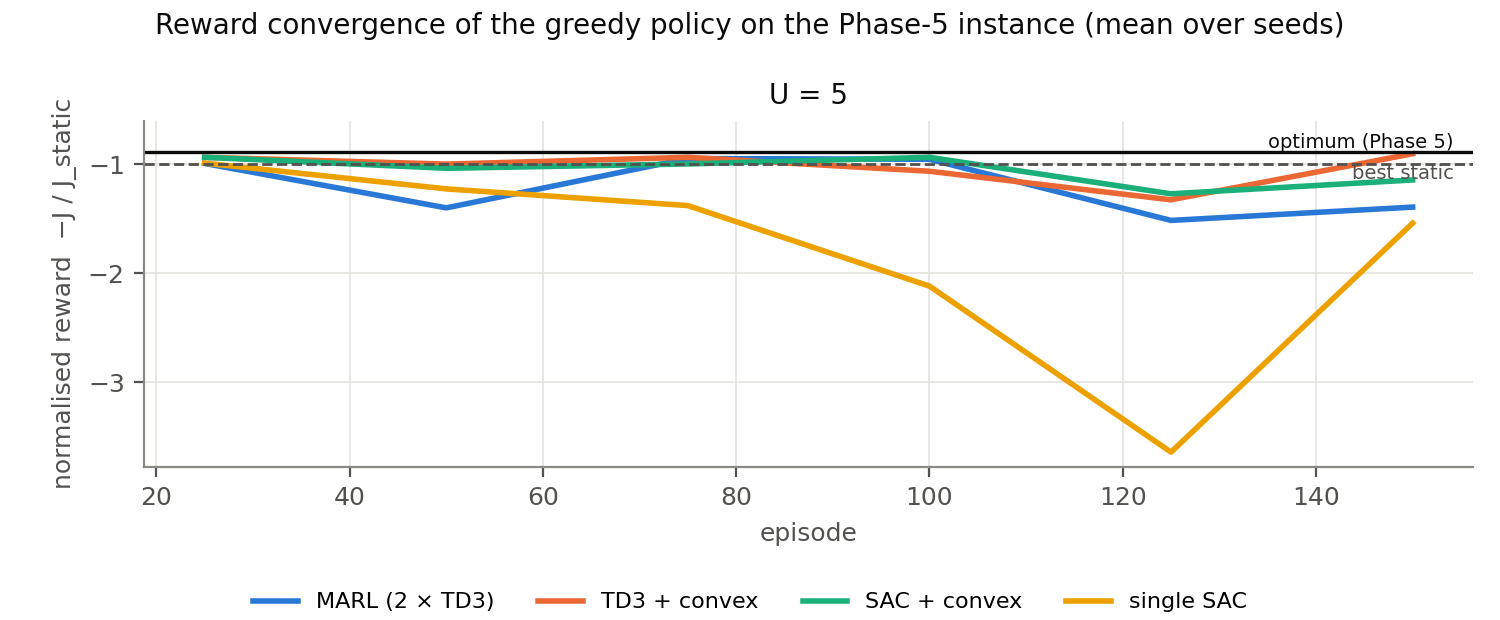
\includegraphics[width=0.75\textwidth]{figures/rl_reward_convergence.png}
	\caption{Normalised reward $-J/J_{\text{static}}$ of the trained policy on the reference instance. Solid line: optimum; dashed: best static (pilot, $U=5$).}\label{fig:rl}
\end{figure}

\begin{itemize}
	\item \textbf{The residual prior is essential.} With it, all four methods beat the best static scenario. Without it, the large agent gets only 10 transitions per episode and spends most of training finding an acceptable configuration from a random start.
	\item \textbf{TD3 + convex is closest to the optimum} (2.2\%). The frequent, continuous part (PRBs and power) is solved exactly, so the agent only has to learn the infrequent discrete decisions.
	\item \textbf{MARL and single SAC also learn PRBs and power}, and are further away and less stable. At $U\ge10$ these agents drift to saturated actions that concentrate resources on a few users and break QoS and queue stability. The share factor $\tau=1$ and the action penalty $c_a$ in~\eqref{eq:reward} counter this. % TODO: report the validated setting
	\item \textbf{Decision time:} one forward pass of the actor (layers 1024 and 512) takes about 2.5\,ms on a single CPU core at $U=20$; the optimisation takes about 47\,min at $U=10$.
\end{itemize}

% =====================================================================================
\section{Summary}\label{sec:summary}
\begin{itemize}
	\item Jointly optimising association, PRBs, power and CU/DU placement lowers the objective by 18--33\% compared with the best static scenario. A certified lower bound backs this up: the conditional gap is below 1.5\%.
	\item Placing functions in the regional cloud pays off more as load grows (edge share 65\%$\to$35\%). Splitting CU and DU is chosen only at high load, for some RUs, because it adds midhaul delay and the scheduling constraint.
	\item Following the slice weights, the optimiser moves resources from mMTC to URLLC and eMBB, cutting URLLC delay by 28--41\%.
	\item Among the RL methods, a large-timescale agent combined with convex small-timescale optimisation comes closest to the optimum, and decides fast enough for online use. % TODO: confirm with the full results
\end{itemize}

\end{document}
